\chapter{Integrale}
\section{Einführung - Stammfunktionen}
\begin{Definition}
  Sei $f$ eine Funktion, die über einem Intervall $I\in\R$ definiert ist. Man nennt jede Funktion $F$, die auf $I$ differenzierbar ist, für die gilt $F'(x)=f(x)$ ,$\forall x\in I$ eine \emph{Stammfunktion} von $f$.\\
  Ist $F$ irgendeine Stammfunktion von $f$, dann ist auch $F(x)+C$ (mit
  konstantem $C$) eine Stammfunktion, denn beim Ableiten fällt $C$ als
  konstanter Summand weg. Jede Funktion hat also unendlich viele
  Stammfunktionen, die sich aber nur um einen konstanten Summanden
  unterscheiden.
\end{Definition}
\begin{Theorem}
  Jede auf $I$ stetige Funktion besitzt eine Stammfunktion über $I$.
\end{Theorem}


\section{Bestimmte Integrale}
\begin{Definition}
  Sei $f$ eine auf einem Intervall $I$ stetige Funktion und zwei reelle Zahlen $a,b\in\I$. Die reelle Zahl,
  dargestellt durch  $\displaystyle{\int_a^b f(t)dt}$ und gegeben durch $F(b)-F(a)$, mit $F$ als beliebige Stammfunktion von $f$, wird bestimmtes Integral von $a$ bis $b$ von $f$ genannt.
  Eine weitere Darstellungsmöglichkeit des bestimmten Integrals sieht folgendermaßen aus:
  \begin{align*}
    \int_{a}^{b} f(x)dx & = \lim\limits_{n \rightarrow \infty} U_n = \lim\limits_{n \rightarrow \infty} s_n\\
                        & = \lim\limits_{n \rightarrow \infty} O_n = \lim\limits_{n \rightarrow \infty} S_n\\
                        & = \lim\limits_{n \rightarrow \infty} \dfrac{b-a}{n}\sum\limits_{k=1}^{n}f\left(\dfrac{b-a}{n}\cdot k\right)
  \end{align*}
  $S_n$ und $O_n$ bezeichnen die Obersumme, wohingegen $s_n$ und $U_n$ die Untersumme bezeichnen.
\end{Definition}
\begin{Bemerkung}
  Der Hauptunterschied zwischen einem bestimmten und einem unbestimmten Integral ist die Existenz (bestimmtes Integral) bzw. das Fehlen
  (unbestimmtes Integral) der Integrationsgrenzen.\\
  Bei einem bestimmten Integral ist die Lösung ein Flächeinhalt, also ein einfacher Zahlenwert.\\
  Bei einem unbestimmten Integral erhält man als Lösung eine (wie soeben eingeführte) Stammfunktion.\\
  Werden feste Integrationsgrenzen angegeben, handelt es sich um ein bestimmtes Integral.
\end{Bemerkung}
\definecolor{lightblu}{rgb}{0,0,0.3}
\definecolor{lightre}{rgb}{0.3,0,0}
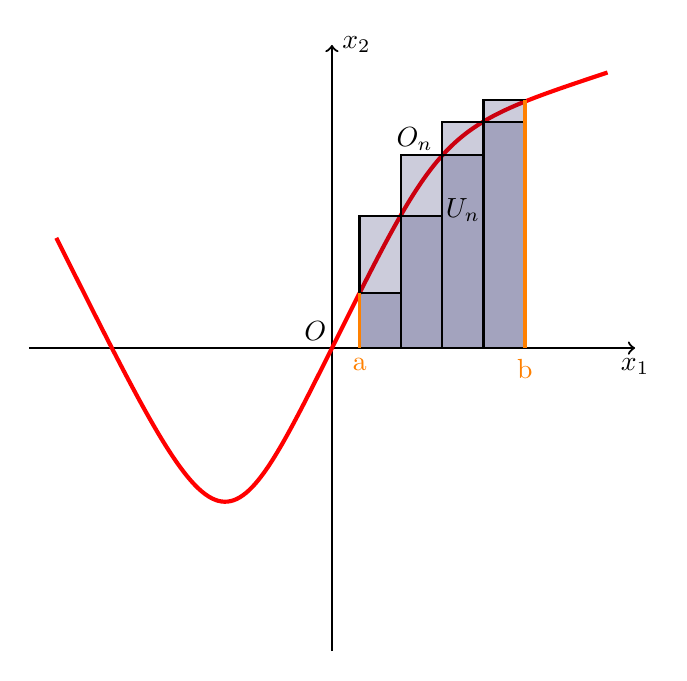
\begin{tikzpicture}[scale=0.7]
  \draw (-0.3,0.3) node {$O$};
  \draw[->,line width=0.8pt] (-5.5,0) -- (5.5,0) node[below] {$x_1$};
  \draw[->,line width=0.8pt] (0,-5.5) -- (0,5.5) node[right] {$x_2$};
  \draw[line width=1.5pt,color=red] (-5,2) ..controls(-2,-4) ..(0,0);
  \draw[line width=1.5pt,color=red] (0,0) ..controls(2,4) ..(5,5);
  \draw[line width=0.8pt,fill=lightblu,fill opacity=0.2] (0.5,0) -- (0.5,2.4) -- (1.25,2.4) -- (1.25,0) -- cycle;
  \draw[line width=0.8pt,fill=lightblu,fill opacity=0.2] (1.25,0) -- (1.25,3.5) -- (2,3.5) -- (2,0) -- cycle;
  \draw[line width=0.8pt,fill=lightblu,fill opacity=0.2] (2,0) -- (2,4.1) -- (2.75,4.1) -- (2.75,0) -- cycle;
  \draw[line width=0.8pt,fill=lightblu,fill opacity=0.2] (2.75,0) -- (2.75,4.5) -- (3.5,4.5) -- (3.5,0) -- cycle;
  \draw[line width=0.8pt,fill=lightblu,fill opacity=0.2] (0.5,0) -- (0.5,1) -- (1.25,1) -- (1.25,0) -- cycle;
  \draw[line width=0.8pt,fill=lightblu,fill opacity=0.2] (1.25,0) -- (1.25,2.4) -- (2,2.4) -- (2,0) -- cycle;
  \draw[line width=0.8pt,fill=lightblu,fill opacity=0.2] (2,0) -- (2,3.5) -- (2.75,3.5) -- (2.75,0) -- cycle;
  \draw[line width=0.8pt,fill=lightblu,fill opacity=0.2] (2.75,0) -- (2.75,4.1) -- (3.5,4.1) -- (3.5,0) -- cycle;
  \draw[line width=1.2pt,color=orange] (0.5,1) -- (0.5,0) node[below] {a};
  \draw[line width=1.2pt,color=orange] (3.5,4.5) -- (3.5,0) node[below] {b};
  \draw (1.5,3.8) node {$O_n$};
  \draw (2.375,2.5) node {$U_n$};
\end{tikzpicture}
\begin{tikzpicture}[scale=0.7]
  \draw[->,line width=0.8pt] (1.5,-7) -- (12.5,-7) node[below] {$x_1$};
  \draw[->,line width=0.8pt] (7,-12.5) -- (7,-1.5) node[right] {$x_2$};
  \draw (6.7,-7.3) node {$O$};
  \draw[line width=1.5pt,color=blue] (2,-9) ..controls(5,-3) ..(7,-4);
  \draw[line width=1.5pt,color=blue] (7,-4) ..controls(10,-5) ..(12,-9);
  \draw[line width=0.8pt,fill=lightre,fill opacity=0.2] (7.5,-7) -- (7.5,-4.2) -- (8.25,-4.2) -- (8.25,-7) -- cycle;
  \draw[line width=0.8pt,fill=lightre,fill opacity=0.2] (8.25,-7) -- (8.25,-4.4) -- (9,-4.4) -- (9,-7) -- cycle;
  \draw[line width=0.8pt,fill=lightre,fill opacity=0.2] (9,-7) -- (9,-4.75) -- (9.75,-4.75) -- (9.75,-7) -- cycle;
  \draw[line width=0.8pt,fill=lightre,fill opacity=0.2] (9.75,-7) -- (9.75,-5.25) -- (10.5,-5.25) -- (10.5,-7) -- cycle;
  \draw[line width=0.8pt,fill=lightre,fill opacity=0.2] (7.5,-7) -- (7.5,-4.4) -- (8.25,-4.4) -- (8.25,-7) -- cycle;
  \draw[line width=0.8pt,fill=lightre,fill opacity=0.2] (8.25,-7) -- (8.25,-4.75) -- (9,-4.75) -- (9,-7) -- cycle;
  \draw[line width=0.8pt,fill=lightre,fillre opacity=0.2] (9,-7) -- (9,-5.25) -- (9.75,-5.25) -- (9.75,-7) -- cycle;
  \draw[line width=0.8pt,fill=lightre,fill opacity=0.2] (9.75,-7) -- (9.75,-6.2) -- (10.5,-6.2) -- (10.5,-7) -- cycle;
  \draw[line width=1.2pt,color=orange] (7.5,-4.2) -- (7.5,0-7) node[below] {a};
  \draw[line width=1.2pt,color=orange] (10.5,-6.2) -- (10.5,-7) node[below] {b};
  \draw (9.5,-4.4) node {$O_n$};
  \draw (8.625,-5.6) node {$U_n$};
\end{tikzpicture}

\begin{Bemerkung}
  $a$ und $b$ bezeichnen jeweils die untere und obere Grenze des zu berechnenden Integrals. Sie bezeichnen anschaulich die $x$-Werte, zwischen denen die Fläche berechnet wird. Tatsächlich ist die geometrische Interpretation von $\displaystyle{\int_a^b f(t)dt}$ die Fläche zwischen dem Schaubild der Funktion und der $x_1$-Achse, die durch die Geraden $x=a$ und $x=b$ begrenzt wird.
\end{Bemerkung}

\begin{Theorem}
  Für eine auf einem Intervall $I$ stetige Funktion $f$ und einer reellen Zahl $a\in I$ gilt: Die Funktion, die über $I$ definiert ist durch $x\mapsto\displaystyle{\int_a^xf(t)dt}$, ist die Stammfunktion von $f$, die bei $a$ gleich $0$ ist.
\end{Theorem}
Aus diesen Sätzen stellt sich der \textbf{Hauptsatz der Differenzial- und Integralrechnung} zusammen. Wir beschränken uns in diesem Kapitel auf die Integralrechnung, da die Differentialrechnung bereits in Kapitel \ref{Funktionsuntersuchung} behandelt wird.\\
\begin{Bemerkung}
  Man beobachtet hier eine Erweiterung der NEW-Regel (siehe \ref{NEW-Regel}, NEW-Regel):\\\\
  \begin{minipage}[b]{0.2\linewidth}
    N $=$ Nullstellen\\
    E $=$ Extremstellen\\
    W $=$ Wendestellen
  \end{minipage}
  \hfill \vline \hfill
  \begin{minipage}[b]{0.4\linewidth}
    \begin{array}{rcccccl}
    F &   N & E & W & & \\
    f & \qquad \qquad& N & E & W & & \\
    f' & \qquad \qquad && N & E & W & \\
    \end{array}
  \end{minipage}
\end{Bemerkung}
\section{Sätze über Integrale}
\begin{Theorem}
\begin{center}
  \begin{tabular}{r c l l}
    \( \displaystyle\int_a^b f(x)dx\) & $=$ &  -\( \displaystyle\int_b^a f(x)dx\) & Invertieren der Intergrationsgrenzen \\
    \( \displaystyle\int_a^b (f(x)+g(x))dx \) & $=$ &  \( \displaystyle\int_a^b f(x)dx + \int_a^b g(x)dx\) & Summenregel\\
    \( \displaystyle\int_a^b r*f(x)dx\)  & $=$ &  \( \displaystyle r*\int_a^b f(x)dx\) & Linearität\\
    \( \displaystyle\int_a^b f(x)dx +\int_b^c f(x)dx\)  & $=$ &  \( \displaystyle\int_a^c f(x)dx\) & Abschnittweise Integration
\end{tabular}

\end{center}
\end{Theorem}
Invertieren der Intergrationsgrenzen:
\begin{Beweis}
  $$\int_a^b f(x)dx = F(b)-F(a) = -(F(a)-F(b)) = -\int_b^a f(x)dx$$
\end{Beweis}
\\
Summenregel:
\begin{Beweis}
  $$\int_a^b f(x)+g(x)dx = [F(x)+G(x)]_a^b = F(b)+G(b)-(F(a)+G(b)) = F(b)-F(a)+G(b)-G(b) $$$$= \int_a^b f(x)dx+\int_a^b g(x)dx$$
\end{Beweis}
\\
Linearität:
\begin{Beweis}
  $$\int_a^b r*f(x)dx = [r*F(x)]_a^b = r*F(b)-r*F(a) = r*(F(a)-F(b)) = r*\int_a^b f(x)dx$$
\end{Beweis}
\\
Abschnittweise Integration:
\begin{Beweis}
  $$\int_a^b f(x)dx+ \int_b^c f(x)dx = F(a)-F(b)-(F(b)-F(c)) = F(c)-F(a) = \int_a^c f(x)dx$$
\end{Beweis}

\begin{Theorem}
  Sei eine in $[a;b]$ stetige Funktion $f$. Wenn für $m,M \in \R$ gilt: $m\leq f(t) \leq M \; \forall t \in [a;b]$, dann gilt:
  $$m(b-a) \leq \int_a^b f(t)dt \leq M(b-a)$$
\end{Theorem}
\begin{Beweis}
  Es reicht, $m \leq f(t) \leq M$ als Ungleichung zwischen $a$ und $b$ zu integrieren.
\end{Beweis}
\begin{minipage}{0.5\linewidth}
  \begin{Bemerkung}
    Eine Konsequenz davon ist, dass falls $|f(t)|\leq M \; \forall t \in [a;b]$, dann gilt:
    $$\left|\int_a^b f(t)dt \right| \leq M(|b-a|)$$
  \end{Bemerkung}
\end{minipage}
\begin{minipage}{0.5\linewidth}
  \begin{center}
    \definecolor{lightblu}{rgb}{0,0,0.3}
    \definecolor{blu}{rgb}{0,0.3,0.3}
    \definecolor{lightgree}{rgb}{0,0.3,0}
    \definecolor{gree}{rgb}{0.1,0.3,0}
    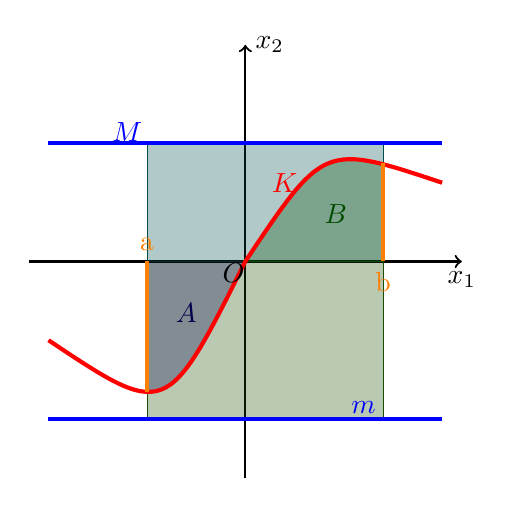
\begin{tikzpicture}[scale=0.50]
        \draw[->,line width=0.8pt] (-5.5,0) -- (5.5,0) node[below] {$x_1$};
        \draw[->,line width=0.8pt] (0,-5.5) -- (0,5.5) node[right] {$x_2$};
        \draw[line width=0.1pt,color=blu,fill=blu,fill opacity=0.3] (-2.5,0) -- (-2.5,3) -- (3.5,3) -- (3.5,0) -- cycle;
        \draw[line width=0.1pt,color=gree,fill=gree,fill opacity=0.3] (-2.5,0) -- (-2.5,-4) -- (3.5,-4) -- (3.5,0) -- cycle;
        \draw[line width=0.1pt,color=lightblu,fill=lightblu,fill opacity=0.3] (-2.5,0) -- (-2.5,-3.32) ..controls(-1.71,-3.25) ..(0,0) -- cycle;
        \draw[line width=0.1pt,color=lightgree,fill=lightgree,fill opacity=0.3] (0,0) ..controls(1.8,2.7) ..(3.5,2.5) -- (3.5,0) -- cycle;
        \draw[line width=1.5pt,color=red] (-5,-2) ..controls(-2,-4) ..(0,0);
        \draw[line width=1.5pt,color=red] (0,0) ..controls(2,3) ..(5,2);
        \draw[line width=1.5pt,color=blue] (-5,3) -- (5,3);
        \draw[line width=1.5pt,color=blue] (-5,-4) -- (5,-4);
        \draw[line width=1.2pt,color=orange] (-2.5,-3.32) -- (-2.5,0) node[above] {a};
        \draw[line width=1.2pt,color=orange] (3.5,2.5) -- (3.5,0) node[below] {b};
        \draw (-0.3,-0.3) node {$O$};
        \draw[line width=0.8pt,color=lightblu] (-1.5,-1.3) node {$A$};
        \draw[line width=0.8pt,color=lightgree] (2.3,1.2) node {$B$};
        \draw[line width=0.8pt,color=red] (1,2) node {$K$};
        \draw[line width=0.8pt,color=blue] (-3,3.3) node {$M$};
        \draw[line width=0.8pt,color=blue] (3,-3.7) node {$m$};
    \end{tikzpicture}
  \end{center}
\end{minipage}

Außerdem:
\begin{Definition}
  Für eine auf $[a;b]$ stetige Funktion $f$ mit $a \neq b$ gilt: Der Mittelwert von $f$ auf $[a;b]$ ist gegeben durch $$\mu = \dfrac{1}{b-a} \int_a^b f(t)dt$$
\end{Definition}

\section{Integrationsregeln und -techniken}

\subsection{Potenzregel}
Hoffentlich einleuchtend und selbstverständlich:
\begin{Theorem}
  $$\forall n \in \Z \textbackslash \{ -1\}:\int  x^n dx = \frac{1}{n+1}x^{n+1} + C$$
\end{Theorem}
\begin{Bemerkung}
  Die einzige Ausnahme stellt der Fall $n=-1$ dar:
\end{Bemerkung}
\begin{Theorem}
  $$\int  \dfrac{1}{x} dx = \ln(|x|) + C$$
\end{Theorem}
Eine Konsequenz dessen ist:
\begin{Theorem}
  $$\int  \dfrac{a}{bx+c} dx = \dfrac{a}{b}\ln(|bx+c|) + C$$
\end{Theorem}
\begin{Beweis}
  So what?
\end{Beweis}

\subsection{Partielle Integration}
\begin{Theorem}
  Seien $u$ und $v$ zwei stetig differenzierbare Funktionen im Intervall $I$ und $u'$
  und $v'$ in I stetig. Dann gilt:
  $$\int u(x)'v(x) dx= u(x)v(x) - \int u(x)v'(x) dx$$
\end{Theorem}
\begin{Beweis}\\
Nachweisen u, v diffbar und u', v' stetig (kommt noch in sauber)\\
\begin{align*}
  &&(u(x)*v(x))' &= u'(x)v(x)+u(x)v'(x)\\
  &\Leftrightarrow & \int (u(x)*v(x))' dx &= \int u'(x)v(x)+\int u(x)v'(x)\\
  &\Leftrightarrow & u(x)*v(x) &= \int u'(x)v(x)+\int u(x)v'(x)\\
  &\Leftrightarrow & \int u(x)v'(x) &= u(x)*v(x)- \int u'(x)v(x)\\
\end{align*}
\end{Beweis}
\begin{Beispiel}
  \begin{align*}
  \int x\sin(x) dx &= \int x(-\cos(x))' dx\\
  &= -x\cos(x) - \int-\cos(x)*1 dx\\
  &= -x\cos(x) + \int\cos(x) dx\\
  &= -x\cos(x) + \sin(x)
\end{align*}
\end{Beispiel}

\subsection{Substitution}
\begin{Theorem}
  Es sei $f$ eine auf $[a;b]$ stetige funktion und $g$ eine auf diesem Intervall differenzierbare Funktion mit stetiger Ableitung
  $g'$. Wenn die verkettung $f \circ g$ esxistiert, gilt:
  $$\int_a^b f(g(x)*g'(x)dx=\int_{g(a)}^{g(b)}f(z)dz$$
\end{Theorem}
Eine abgespeckte Variante dieses Theorems, genannt lineare Substitution ist gegeben durch:
\begin{Theorem}
  Für ein Funktion $f$ mit einer Stammfunktion $F$ und $r\neq 0$ gilt:
  $$\int_a^b f(rx+s)dx=\dfrac{1}{r}[F(rx+s)]_a^b$$
\end{Theorem}
\begin{Beispiel}
    Zu berechnen: $$\int_0^4 \dfrac{x\sqrt{x}}{1 + x^2\sqrt{x}} dx$$ \\
    \textbf{Substitution}:
    \begin{align*}
        \quad \qquad \qquad \qquad \qquad \qquad u &= x^2\sqrt{x} \quad (\text{alternativ } u = x^2\sqrt{x} + 1) \\
                                    \dfrac{du}{dx} &= (x^2\sqrt{x})' \\
                                                   &= \dfrac{5}{2} \cdot x\sqrt{x} \\
                                \Leftrightarrow dx &= \dfrac{2}{5x\sqrt{x}}du
    \end{align*}
    \textbf{Berechnung des Integrals}:
    \begin{align*}
        \int_0^4 \dfrac{x\sqrt{x}}{1 + x^2\sqrt{x}} dx &= \int_{u(0)}^{u(4)} \dfrac{\cancel{x\sqrt{x}}}{1 + u} \cdot \dfrac{2}{5\cancel{x\sqrt{x}}}du \\
                                                       &= \dfrac{2}{5} \cdot \int_{0^2\sqrt{0}}^{4^2\sqrt{4}} \dfrac{1}{1 + u}du \\
                                                       &= \dfrac{2}{5} \cdot \left[\ln(|1 + u|)\right]_0^{32} \\
                                                       &\boxed{= \dfrac{2}{5} \cdot \ln(33)}
    \end{align*}
\end{Beispiel}

\subsection{Substitution der Integrationsvariablen}
\begin{Theorem}
  Es sei $f$ eine auf $[a;b]$ stetige funktion und $g$ eine auf diesem Intervall differenzierbare und umkehrbare Funktion mit stetiger
  Ableitungsfunktion $g'$. Wenn die verkettung $f \circ g$ esxistiert, gilt:
  $$\int_a^b f(x)dx=\int_{\bar g (a)}^{\bar g (b)}f(g(t))*g'(t)dt$$
\end{Theorem}

\subsection{Partialbruchzerlegung}
?

\subsection{Integrale von $e$-Funktionen}
\begin{Theorem}
  Für $f(x)=e^{l(x)}$ mit $l(x) = ax+b$ gilt: $F(x) = \dfrac{1}{a}e^{l(x)}$
\end{Theorem}
\begin{Beweis}
  Man bilde $F'(x)$.
\end{Beweis}
\subsection{Integrale von $\ln()$-Funktionen}
Es handelt sich hierbei streng genommen auch um eine Substitution:
\begin{Theorem}
  Für $x \in \R^{+}$ ist $F$ eine Stammfunktion zur Funktion $f(x) = \ln(x)$ mit $F(x) = x \ln(x)-x$
\end{Theorem}
\begin{Beweis}
  Der Beweis erfolgt über partielle Integration und wird dem Schüler als Übung überlassen.
\end{Beweis}
\subsection{Integrale von (un)geraden Funktionen}
\begin{Theorem}
  Sei $f$ eine auf einem Intervall $I$ stetige und auf $0$ zentrierte Funktion. Wenn $f$ gerade ist, gilt für alle $a\in \R$:
  $\displaystyle{\int_{-a}^{a} f(t)dt = 2\int_{0}^{a} f(t)dt } $, und wenn $f$ ungerade ist
  $\( \displaystyle\int_{-a}^{a} f(t)dt = 0 \) $
\end{Theorem}
\begin{Beweis}
  Sei die Funktion $\varphi(x) = \( \displaystyle\int_{-x}^{x}f(t)dt = F(x)-F(-x)$ mit $F$, einer Stammfunktion von $f$. Also ist $\varphi$ auf
  $I = [-x;x]$ differenzierbar und $\varphi'(x) = F'(x)-F'(-x)=f(x)+f(-x)$.\\
  Wenn $f$ auf $I$ ungerade ist, gilt: $\varphi'(x) = 0$ und somit konstant (und außerdem $=\varphi(x)$) auf $I$, was $\( \displaystyle\int_{-a}^{a} f(t)dt = 0$ beweist.\\
  Wenn $f$ gerade ist, gilt: $\varphi'(x) = 2f(x)$. Also gilt für $\varphi(x)=\displaystyle{\int_0^x 2f(t)dt}$, einer Stammfunktion von $2f(x)$,  $\varphi(0)=0$, was $\displaystyle{\int_{-a}^{a} f(t)dt = 2\int_{0}^{a} f(t)dt }$ beweist.
\end{Beweis}
\subsection{Integrale von periodischen Funktionen}
\begin{Theorem}
  Für jede auf $\R$ stetige und periodische Funktion $f$ gilt:
  \begin{center}
  \( \displaystyle\int_a^{a+T} f(x)dx\) ist unabhängig von $a$ und \( \displaystyle\int_a^{a+T} f(x)dx = \int_0^{T} f(x)dx\)
  \end{center}
\end{Theorem}
\begin{Beweis}
  Sei die Funktion $\varphi = \displaystyle{\int_x^{x+T} f(t)dt}=F(x+T)-F(x)$ mit $F$, einer Stammfunktion von $f$. Dann ist
  $\varphi(x)$ auf $f$ differenzierbar und $\varphi'(x)=F'(x+T)-F'(x) = f(x+T)-f(x)=0$ (denn $f$ hat die Periode $T$). Also ist $\varphi(x)$ auf $\R$ konstant. Daraus folgt, dass $\displaystyle{\int_a^{a+T}f(t)dt}$ nicht von $a$ abhängt und dass $\displaystyle{\int_a^{a+T} f(x)dx = \int_0^{T} f(x)dx}$.
\end{Beweis}


\section{Flächen und Volumen mit Integralen berechnen}

\subsection{Fläche zwischen einer Funktion und der $x_1$-Achse}
\begin{Definition}
  Für die auf dem Intervall $[a;b]$ (also stückweise) stetige Funktion $f$ mit Nullstellen und $x_1,x_2,...,x_n$
  mit $a \leq x_1 \leq x_2 \leq ... \leq x_n \leq b$ ist der Flächeninhalt $A$ zwischen dem Graphen von $f$ und
  der $x_1$-Achse im Intervall $[a;b]$ gegeben durch:
  $$A= \left|{\int_a^{x_1} f(x)dx}\right|+\left|{\int_{x_1}^{x_2} f(x)dx}\right|+...+\left|{\int_{x_{n-1}}^{x_n} f(x)dx}\right|+\left|{\int_{x_n}^b f(x)dx}\right|$$
\end{Definition}
Bildhaft sieht das folgendermaßen aus:
\begin{center}
    \definecolor{lightblu}{rgb}{0,0,0.3}
    \definecolor{lightgree}{rgb}{0,0.3,0}
    \begin{tikzpicture}[scale=0.7]
        \draw[->,line width=0.8pt] (-5.5,0) -- (5.5,0) node[below] {$x_1$};
        \draw[->,line width=0.8pt] (0,-5.5) -- (0,5.5) node[right] {$x_2$};
        \draw[line width=0.1pt,color=lightblu,fill=lightblu,fill opacity=0.3] (-2.5,0) -- (-2.5,-2.5) ..controls(-1.62,-3.072) ..(0,0) -- cycle;
        \draw[line width=0.1pt,color=lightgree,fill=lightgree,fill opacity=0.3] (0,0) ..controls(1.94,3.78) ..(3.5,4.5) -- (3.5,0) -- cycle;
        \draw[line width=1.5pt,color=red] (-5,2) ..controls(-2,-4) ..(0,0);
        \draw[line width=1.5pt,color=red] (0,0) ..controls(2,4) ..(5,5);
        \draw[line width=1.2pt,color=orange] (-2.5,-2.5) -- (-2.5,0) node[above] {a};
        \draw[line width=1.2pt,color=orange] (0,-0.2) node[right] {$x_1$};
        \draw[line width=1.2pt,color=orange] (3.5,4.5) -- (3.5,0) node[below] {b};
        \draw[line width=1.2pt,color=orange] (-2.5,-1.5) -- (-1,0);
        \draw[line width=1.2pt,color=orange] (-2.5,-0.5) -- (-2,0);
        \draw[line width=1.2pt,color=orange] (-2.5,-2.5) -- (3.5,3.5);
        \draw[line width=1.2pt,color=orange] (1,0) -- (3.5,2.5);
        \draw[line width=1.2pt,color=orange] (2,0) -- (3.5,1.5);
        \draw[line width=1.2pt,color=orange] (3,0) -- (3.5,0.5);
        \draw[line width=1.2pt,color=orange] (1,2) -- (3.5,4.45);
        \draw[line width=1.2pt,color=black] (5.5,-2) -- (7.5,-2) -- (7.5,-3) -- (5.5,-3) -- cycle;
        \draw[line width=1.2pt,color=orange] (5.5,-3) -- (6.5,-2);
        \draw[line width=1.2pt,color=orange] (6.5,-3) -- (7.5,-2);
        \draw[line width=1.2pt,color=orange] (5.5,-2.5) -- (6,-2);
        \draw[line width=1.2pt,color=orange] (6,-3) -- (7,-2);
        \draw[line width=1.2pt,color=orange] (7,-3) -- (7.5,-2.5);
        \draw[line width=3pt] (7.8,-2.5) node {:};
        \draw[line width=2pt] (9,-2.5) node {$\textcolor{orange}{C} = \textcolor{lightblue}{A} + \textcolor{lightgree}{B}$};
        \draw[line width=2pt] (10.75,-3) node {$ = |{\int_{\textcolor{orange}{a}}^{\textcolor{orange}{x_1}} f(x)dx}| + |{\int_{\textcolor{orange}{x_1}}^{\textcolor{orange}{b}} f(x)dx}|$};
        \draw (-0.3,-0.3) node {$O$};
        \draw[line width=0.8pt,color=lightblu] (-1.5,-1.1) node {$A$};
        \draw[line width=0.8pt,color=lightgree] (2.3,1.9) node {$B$};
        \draw[line width=0.8pt,color=red] (2,4) node {$K$};
    \end{tikzpicture}
\end{center}
\\
\begin{Beispiel}
  $f(x)=x^2-2x^3;x\in \R$\\
  notwendige und hinreichende Bedingung für Nullstellen:$f(x)=0$\\
  $\Leftrightarrow x^2(1-2x)&=0\\
  \stackrel{SdN}{\Leftrightarrow}
  \left\{ \begin{array}{rcl}
  x^2&=0\\
  1-2x&=0
  \end{array}\right\\
  \Leftrightarrow
  \left\{ \begin{array}{rcl}
  x_1&=0\\
  x_2&=\dfrac{1}{2}
  \end{array}\right\\
  $\\
  Also gilt:\\
  \begin{align*}
    A_{-1}^{1} &= \left|\int_{-1}^0 x^2-2x^3 dx\right| + \left|\int_{0}^{0.5} x^2-2x^3 dx\right| + \left|\int_{0.5}^1 x^2-2x^3 dx\right|\\
    &= \left|\left[\dfrac{1}{3}x^3-\dfrac{1}{2}x^4\right]_{-1}^0\right| + \left|\left[\dfrac{1}{3}x^3-\dfrac{1}{2}x^4\right]_{0}^{0.5}\right| + \left|\left[\dfrac{1}{3}x^3-\dfrac{1}{2}x^4\right]_{0.5}^1\right|\\
    &= \left|0-\left(-\dfrac{1}{3}-\dfrac{1}{2}\right)\right| + \left|\dfrac{1}{24}-\dfrac{1}{32}-0\right| + \left|\dfrac{1}{3}-\dfrac{1}{2}- \left(\dfrac{1}{24}-\dfrac{1}{32}\right)\right|\\
    &= 1 + \dfrac {1}{12} - \dfrac{1}{16}\\
    &= \dfrac{49}{48} \text{  FE}
\end{align*}
\end{Beispiel}
\begin{GTR-Tipp}
  Mit $Y_1 = f(x)$ und $Y_2 = abs(Y_1)$ bzw. $Y_2 = |Y_1|$ (zu finden in 'MATH'>'NUM' oder über Alpha-F2) lässt sich die Fläche berechnen über 2nd-CALC mit der Option Integral.\\
  Hierzu wählt man $Y_2$ aus und gibt $a$ und $b$ an.
\end{GTR-Tipp}
\begin{center}
    \definecolor{lightblu}{rgb}{0,0,0.3}
    \definecolor{lightgree}{rgb}{0,0.3,0}
    \begin{tikzpicture}[scale=0.7]
        \draw[->,line width=0.8pt] (-5.5,0) -- (5.5,0) node[below] {$x_1$};
        \draw[->,line width=0.8pt] (0,-5.5) -- (0,5.5) node[right] {$x_2$};
        \draw[line width=0.1pt,color=lightblu,fill=lightblu,fill opacity=0.3] (-2.5,0) -- (-2.5,2.43) ..controls(-1.59,3.21) ..(0,0) -- cycle;
        \draw[line width=0.1pt,color=lightgree,fill=lightgree,fill opacity=0.3] (0,0) ..controls(1.94,3.78) ..(3.5,4.5) -- (3.5,0) -- cycle;
        \draw[line width=1.5pt,color=red] (-5,2) ..controls(-2,-4) ..(0,0);
        \draw[line width=1.5pt,color=red] (0,0) ..controls(2,4) ..(5,5);
        \draw[line width=1.5pt,color=red] (-4,0) ..controls(-1.8,3.8) ..(0,0);
        \draw[line width=7pt,color=white,dashed] (-4,0) ..controls(-1.8,-3.8) ..(0,0);
        % Repair the damage caused by the line above
        \draw[line width=0.8pt] (-4,0) -- (-3.85,0);
        \draw[line width=0.8pt] (0,-0.05) -- (0,-0.3);
        \draw[line width=1.2pt,color=orange] (-2.5,2.4) -- (-2.5,0) node[below] {a};
        \draw[line width=1.2pt,color=orange] (0,-0.2) node[right] {$x_1$};
        \draw[line width=1.2pt,color=orange] (3.5,4.5) -- (3.5,0) node[below] {b};
        \draw[line width=1.2pt,color=orange] (-2.5,0.5) -- (-1,2);
        \draw[line width=1.2pt,color=orange] (-2.5,1.5) -- (-1.4,2.6);
        \draw[line width=1.2pt,color=orange] (-2,0) -- (-0.65,1.35);
        \draw[line width=1.2pt,color=orange] (-1,0) -- (-0.3,0.7);
        \draw[line width=1.2pt,color=orange] (0,0) -- (3.5,3.5);
        \draw[line width=1.2pt,color=orange] (1,0) -- (3.5,2.5);
        \draw[line width=1.2pt,color=orange] (2,0) -- (3.5,1.5);
        \draw[line width=1.2pt,color=orange] (3,0) -- (3.5,0.5);
        \draw[line width=1.2pt,color=orange] (1,2) -- (3.5,4.45);
        \draw[line width=1.2pt,color=black] (5.5,-2) -- (7.5,-2) -- (7.5,-3) -- (5.5,-3) -- cycle;
        \draw[line width=1.2pt,color=orange] (5.5,-3) -- (6.5,-2);
        \draw[line width=1.2pt,color=orange] (6.5,-3) -- (7.5,-2);
        \draw[line width=1.2pt,color=orange] (5.5,-2.5) -- (6,-2);
        \draw[line width=1.2pt,color=orange] (6,-3) -- (7,-2);
        \draw[line width=1.2pt,color=orange] (7,-3) -- (7.5,-2.5);
        \draw[line width=3pt] (7.8,-2.5) node {:};
        \draw[line width=2pt] (9,-2.5) node {$\textcolor{orange}{C} = \textcolor{lightblue}{A} + \textcolor{lightgree}{B}$};
        \draw[line width=2pt] (10.57,-3.05) node {$ = {\int_{\textcolor{orange}{a}}^{\textcolor{orange}{x_1}} f(x)dx} + {\int_{\textcolor{orange}{x_1}}^{\textcolor{orange}{b}} f(x)dx}$};
        \draw[line width=2pt] (9.47,-3.6) node {$ = {\int_{\textcolor{orange}{a}}^{\textcolor{orange}{b}} f(x)dx}$};
        \draw (-0.3,-0.3) node {$O$};
        \draw[line width=0.8pt,color=lightblu] (-1.5,1.1) node {$A$};
        \draw[line width=0.8pt,color=lightgree] (2.3,1.9) node {$B$};
        \draw[line width=0.8pt,color=red] (1.45,4.05) node{"$ $};
        \draw[line width=0.8pt,color=red] (1.8,4) node {$|K|$};
        \draw[line width=0.8pt,color=red] (2.15,4.05) node{"$ $};
    \end{tikzpicture}
\end{center}
\subsection{Fläche zwischen zwei Funktionen}
\begin{Theorem}
  Für zwei auf $[a;b]$ stetige Funktionen $f$ und $g$ gilt: Die Fläche zwischen ihren Schaubildern $C_f$ und $C_g$ ist gegeben durch: $\( \displaystyle \int_a^b (g(x)-f(x))dx$\).
\end{Theorem}
\subsection{Volumenangaben mittels Integralen}
\begin{Theorem}
  Man betrachtet einen Körper, der durch zwei parallele Ebenen mit den Gleichungen $x_3 = a$ und $x_3 = b$ begrenzt wird.
  Für alle $a\leq z \leq b$ nennt man $P_z$ die orthogonale Fläche zu $x_3$-Achse mit der Seite $z$ und $S(z)$ die Fläche des
  Schnitts des Körpers durch $P_z$. Ist $S$ stetig, so ist ist das Volumen $V$ des Körpers gegeben durch:
  $$V=\int_a^b S(z)dz$$\\
\end{Theorem}
\begin{Bemerkung}
  Dieses Theorem nehmen wir hin, ohne es zu beweisen, uns geht es ohnehin um die Schlussfolgerungen, die wir daraus ziehen können:
\end{Bemerkung}
\begin{Theorem}
  Ein Körper, der durch die Rotation der Kurve von $f$ um die $x_1$-Achse entsteht, hat ein Volumen von
  \( \displaystyle \pi \int_a^b f^2(z)dz\).\\
  Tatsächlich ist die Fläche eines zur $x_3$-Achse parallelen Querschnitts die der Scheibe mit Radius $f(z)$.
\end{Theorem}
\definecolor{ffqqqq}{rgb}{1,0,0}
\definecolor{ccqqqq}{rgb}{0.8,0,0}
\begin{tikzpicture}[line cap=round,line join=round,>=triangle 45,x=1cm,y=1cm,scale=0.7]
  \draw[->,line width=0.8pt] (-3.0,0) -- (11.0,0) node[below] {$x_1$};
  \draw[->,line width=0.8pt] (0,-3.7) -- (0,3.7) node[right] {$x_2$};
  \draw[->,line width=0.8pt] (-3.0,-3.0) -- (3.0,3.0) node[right] {$x_3$};
  \draw (-0.3,0.3) node {$O$};
  \draw[line width=2.4pt,color=ffqqqq,fill=ffqqqq,fill opacity=0.1, smooth,samples=50,domain=1:9] plot(\x,{sqrt(\x)}) -- (9,0) -- (1,0) -- cycle;
  \draw[line width=2pt,color=ccqqqq,smooth,samples=100,domain=6.848866262443662e-8:10.024582490069186] plot(\x,{sqrt((\x))});
  \draw[line width=2.4pt,dash pattern=on 1pt off 1pt,color=ffqqqq,smooth,samples=100,domain=6.848866262443662e-8:10.024582490069186] plot(\x,{0-sqrt((\x))});
  \draw [rotate around={90:(1,0)},line width=1pt] (1,0) ellipse (1.0085893502642513cm and 0.13134868658068935cm);
  \draw [rotate around={90:(9,0)},line width=1pt] (9,0) ellipse (3.0174458893236813cm and 0.32400570210806623cm);
\end{tikzpicture}
\section{Uneigentliche Integrale}
\begin{Definition}
  Ist die Funktion $f$ auf $[a;+\infty)$ stetig und existiert der Grenzwert \( \displaystyle\lim\limits_{Z \rightarrow \infty} \int_a^Z f(x)dx\),
  so heißt dieser Grenzwert \emph{uneigentliches Integral} von $f$ über $[a;+\infty)$.\\
  Schreibweise: \( \displaystyle\int_a^{+\infty} f(x)dx\)\\
  Analog dazu spricht man von einem uneigentlichen Integral für \( \displaystyle\int_{-\infty}^b f(x)dx\)
\end{Definition}
\begin{Beispiel}
  $f(x)=\dfrac{-3}{x^3}$\\
  \( \displaystyle A(z)=\int_z^{-2} \dfrac{-3}{x^3} dx = \left[\dfrac{3}{2}x^{-2}\right]_z^{-2} = \dfrac{3}{8}-\dfrac{3}{2}z^{-2}\)\\
  $\lim \limits_{z \rightarrow -\infty} \dfrac{3}{8}-\dfrac{3}{2}z^{-2} = \dfrac{3}{8}$\\
  $\Rightarrow$ Das uneigentliche Integral hat den Wert $\dfrac{3}{8}$.
\end{Beispiel}
\begin{Beispiel}
  $f(x)=\dfrac{1}{\sqrt x}$\\
  \( \displaystyle A(z)=\int_z1^{Z} \dfrac{1}{\sqrt x} dx = \left[2\sqrt x \right]_1^{Z} = 2\sqrt Z - 2\)\\
  $\lim \limits_{Z \rightarrow \infty} 2\sqrt Z - 2 \stackrel{\rightarrow}{Z \rightarrow \infty} \infty$\\
  $\Rightarrow$ Das uneigentliche Integral existiert nicht.
\end{Beispiel}
\begin{Definition}
  Ist die Funktion $f$ auf $(a;b]$ stetig und existiert der Grenzwert \( \displaystyle\lim\limits_{Z \rightarrow a} \int_Z^b f(x)dx\),
  so heißt dieser Grenzwert \emph{uneigentliches Integral} von $f$ über $(a;b]$.\\
  Schreibweise: \( \displaystyle\int_a^b f(x)dx\)\\
  Analog dazu spricht man von einem uneigentlichen Integral für \( \displaystyle\int_{c}^a f(x)dx\)
\end{Definition}
\begin{Bemerkung}
  Diese Berechnung ergibt nur dann Sinn, wenn bei $a$ eine Definitionslücke vorliegt.
\end{Bemerkung}
\section{Merkenswerte Integrale}
Hier eine (möglicherweise unvollständige) rückblickende Liste mit Integralen, die insbesondere zum Abitur beherrscht werden sollten.\\
Diese sollten ohne weitere Rechtfertigung oder Beweis verwendet werden dürfen. (Diese Angabe ist ohne Gewähr)\\
\begin{align*}
  \int x^n dx &=\dfrac{x^{n+1}}{n+1} + C\\
  \int\dfrac{1}{x} dx &= \ln(|x|) + C\\
  \int\sin x dx &= -\cos x + C\\
  \int\cos x dx &= \sin x + C\\
  \int\dfrac{1}{\cos^2x}dx &= \tan x + C\\
  \int\dfrac{1}{\sqrt{x}}dx &= 2\sqrt{x} + C\\
  \int\dfrac{u'(x)}{u(x)} dx &= \ln(|u(x)|) + C\\
  \int e^{ax+b}dx &= \dfrac{1}{a}e^{ax+b} + C\\
  \int \dfrac{1}{\sqrt x} &= 2\sqrtx + C\\
\end{align*}
\danger Definitionsmengen sind zu beachten.
